\documentclass[tikz,border=2pt]{standalone}
% Shared look for the paper's diagrams (built standalone: figures/diagrams/Makefile).
\usepackage[T1]{fontenc}
\usepackage{newtxtext,newtxmath}
\usepackage{xcolor}
\usepackage{tikz}
\usetikzlibrary{positioning,arrows.meta,fit,calc,backgrounds,decorations.pathreplacing}
\definecolor{ink}{HTML}{1F2328}
\definecolor{muted}{HTML}{6A737D}
\definecolor{rulec}{HTML}{D0D4DC}
\definecolor{fillc}{HTML}{F4F5F8}
\definecolor{sone}{HTML}{2A78D6}   % categorical slot 1: Kubernetes Job / trees
\definecolor{stwo}{HTML}{EB6834}   % slot 2: language models
\definecolor{sthree}{HTML}{1BAF7A} % slot 3: combinations
\definecolor{flyte}{HTML}{6250D6}
\tikzset{
  >={Stealth[length=5pt,width=4pt]},
  every node/.style={font=\small, text=ink},
  box/.style={draw=rulec, fill=white, rounded corners=2pt, inner sep=5pt, line width=0.6pt, align=left},
  head/.style={font=\scriptsize\bfseries\sffamily, text=muted},
  note/.style={font=\scriptsize, text=muted, align=left},
  flow/.style={->, draw=muted, line width=0.7pt},
}

\begin{document}
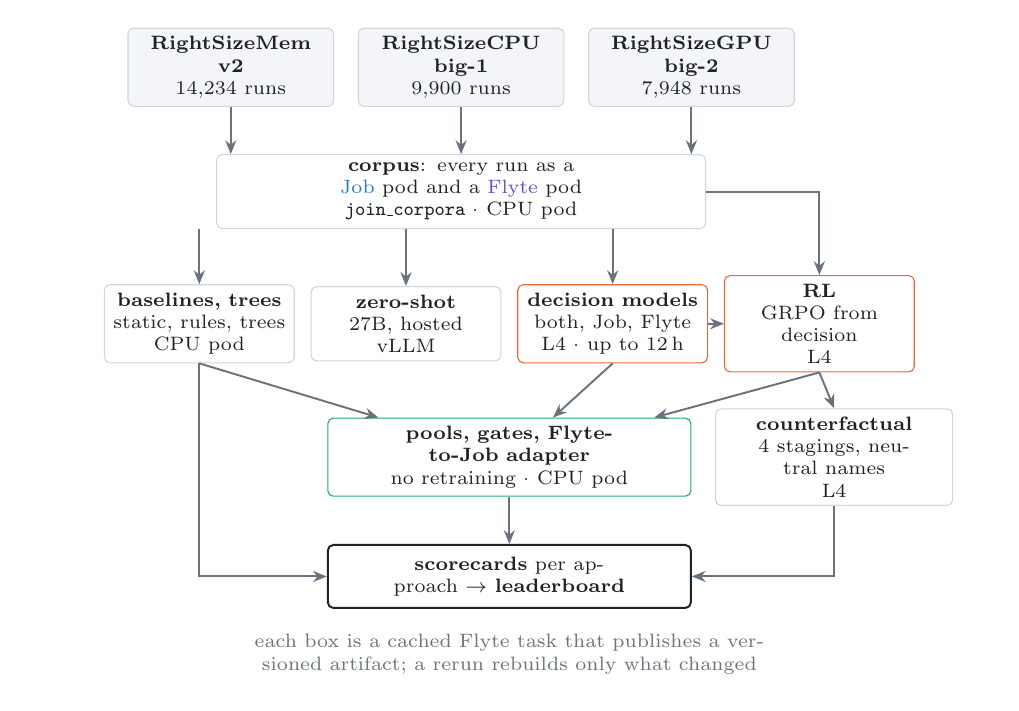
\begin{tikzpicture}[
  art/.style={draw=rulec, fill=white, rounded corners=2pt, inner sep=3pt, align=center, font=\scriptsize, minimum height=8mm},
  src/.style={art, fill=fillc},
  lab/.style={font=\tiny\ttfamily, text=muted},
]
\node[src, text width=24mm] (mem) at (0,0) {\textbf{RightSizeMem v2}\\14,234 runs};
\node[src, text width=24mm, right=3mm of mem] (cpu) {\textbf{RightSizeCPU big-1}\\9,900 runs};
\node[src, text width=24mm, right=3mm of cpu] (gpu) {\textbf{RightSizeGPU big-2}\\7,948 runs};
\node[art, text width=60mm, below=6mm of cpu] (corpus) {\textbf{corpus}: every run as a {\color{sone}Job} pod and a {\color{flyte}Flyte} pod\\ \texttt{join\_corpora} \textperiodcentered\ CPU pod};
\foreach \n in {mem,cpu,gpu} \draw[flow] (\n.south) -- (\n.south |- corpus.north);

\node[art, text width=22mm, below left=7mm and -10mm of corpus.south west] (rules) {\textbf{baselines, trees}\\static, rules, trees\\CPU pod};
\node[art, text width=22mm, right=2mm of rules] (zs) {\textbf{zero-shot}\\27B, hosted vLLM};
\node[art, text width=22mm, right=2mm of zs, draw=stwo] (dec) {\textbf{decision models}\\both, Job, Flyte\\L4 \textperiodcentered\ up to 12\,h};
\node[art, text width=22mm, right=2mm of dec, draw=stwo] (rl) {\textbf{RL}\\GRPO from decision\\L4};
\foreach \n in {rules,zs,dec} \draw[flow] (corpus.south -| \n.north) -- (\n.north);
\draw[flow] (dec) -- (rl);
\draw[flow] (corpus.east) -| (rl.north);

\node[art, text width=44mm, below=7mm of $(zs.south)!0.5!(dec.south)$, draw=sthree] (pool) {\textbf{pools, gates, Flyte-to-Job adapter}\\no retraining \textperiodcentered\ CPU pod};
\node[art, text width=28mm, right=3mm of pool] (cf) {\textbf{counterfactual}\\4 stagings, neutral names\\L4};
\foreach \n in {rules,dec,rl} \draw[flow] (\n.south) -- (pool);
\draw[flow] (rl.south) -- (cf.north);
\node[art, text width=44mm, below=6mm of pool, draw=ink, line width=0.7pt] (board) {\textbf{scorecards} per approach $\to$ \textbf{leaderboard}};
\draw[flow] (pool) -- (board);
\draw[flow] (cf.south) |- (board.east);
\draw[flow] (rules.south) |- (board.west);
\node[note, below=2mm of board, text width=120mm, align=center] {each box is a cached Flyte task that publishes a versioned artifact; a rerun rebuilds only what changed};
\end{tikzpicture}
\end{document}
